\Needspace{20\baselineskip}
\section{系统时间线与内核指标采集}
\label{l14:sec:collection}

\subsection{在统一时间轴上定位耗时}

系统级分析将 CPU 活动、CUDA 应用程序接口（application programming interface，API）调用、GPU 内核和数据传输标在统一的时间轴上。它能区分几种表面上都表现为“程序很慢”的情况：主机尚未提交工作，GPU 正在搬运数据，目标内核本身运行较久，或者某个同步点正在等待前面的工作完成。统计视图给出调用次数、累计时间、平均时间等信息，时间线则展示这些事件之间的重叠和先后关系。

图\ref{l14:fig:nsys}中，主机上的流同步调用 \code{cudaStreamSynchronize} 与 GPU 上连续执行的矩阵乘法重叠。该调用的长区间表示主机在等待指定流完成；沿同一时间轴观察 GPU，才能判断等待期间发生了什么。若直接把主机同步累计时间与 GPU 内核累计时间相加，同一段真实经过的时间就可能被重复计算。

\begin{figure}[htbp]
\centering
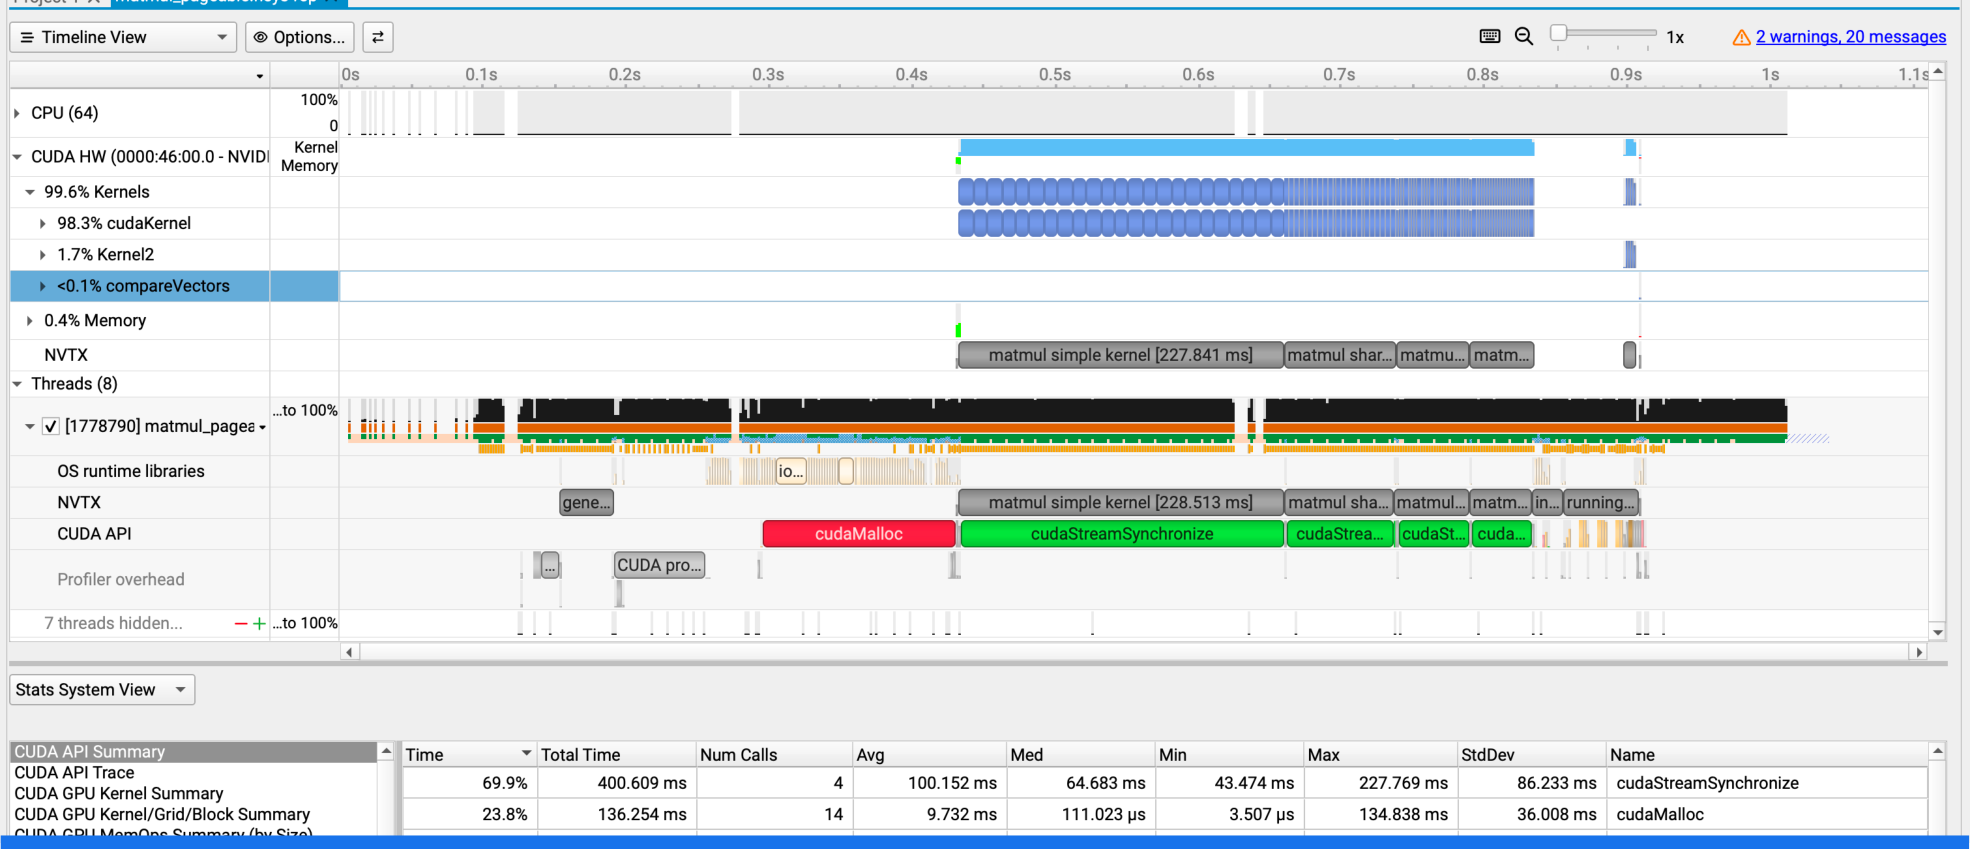
\includegraphics[width=\textwidth]{nsys_timeline.png}
\caption{主机、CUDA 接口和 GPU 活动的统一时间线。同步函数在主机侧持续等待的同时，设备侧可以连续执行多个内核；区间长度需要结合所属轨道解释。}
\label{l14:fig:nsys}
\end{figure}

分析时可以先观察最长区间，再检查其中的结构。若多个短内核之间有明显空隙，应查看主机提交、同步和数据准备；若一段传输之后才开始计算，应检查依赖是否允许重叠；若单个内核占据主要时间，就适合进入内核级分析。内存分配也可能是显著的一次性开销，反复测试时应明确它是否属于目标应用的正常路径。

厂商工具扩展接口（NVIDIA Tools Extension，NVTX）允许程序为主机代码区间命名。命名区间能把“初始化”“矩阵乘法”“结果校验”等阶段对应到时间线。主机区间的结束通常只说明该段主机代码已执行完；如果其中只提交了异步 GPU 工作，设备执行可能延续到区间之后。命名区间、GPU 上对应活动及同步事件需要共同解释。

\subsection{系统级采集命令与报告}

远端采集与本地查看可以分开完成：在具有目标 GPU 的机器上运行命令行采集器 \code{nsys}，生成 \code{.nsys-rep} 报告，再用图形客户端 \code{nsys-ui} 打开。查看已有报告不需要在本地重新执行同一个 GPU 内核。一次普通采集可写成：

\noindent\begin{minipage}{\linewidth}
\begin{lstlisting}[style=cuda,language=bash,numbers=none,caption={系统级采集与报告查看}]
nsys profile --trace=cuda,nvtx,osrt \
  --output=gemm_system --force-overwrite=true ./gemm_demo
nsys-ui gemm_system.nsys-rep
\end{lstlisting}
\end{minipage}

其中 \code{profile} 启动待测程序并按指定范围采集。\code{--trace} 选择 CUDA、命名区间和操作系统运行时等事件；\code{--output} 指定报告文件名的主体；\code{--force-overwrite=true} 允许覆盖同名报告。命令行中的续行符必须位于物理行末，后面不应再接注释。

\begin{table}[htbp]
\centering\small
\caption{系统级采集的常用控制选项}
\label{l14:tab:nsys-options}
\begin{tabularx}{\textwidth}{@{}p{52mm}Y@{}}
\toprule
选项 & 用途\\
\midrule
\code{-o}、\code{--output} & 设置输出报告名称\\
\code{-f}、\code{--force-overwrite} & 控制是否覆盖已有报告\\
\code{-e}、\code{--env-var} & 为被分析程序设置环境变量\\
\code{-y}、\code{--delay} & 延迟指定秒数后开始采集，适合略过已知的启动阶段\\
\code{--capture-range=nvtx} & 用指定的 NVTX 区间控制采集范围\\
\code{-p}、\code{--nvtx-capture} & 选择 NVTX 区间；需要同时启用相应范围控制\\
\code{--stats=true} & 采集后生成统计摘要；数据库导出和统计会增加分析时间\\
\bottomrule
\end{tabularx}
\end{table}

对较复杂的程序，交互模式把启动和采样控制分开：\code{launch} 在适合分析的环境中启动程序，\code{start} 与 \code{stop} 控制采样开始和结束，\code{shutdown} 结束分析会话。提供 \code{cancel} 的版本可以用它取消采集并丢弃尚未保留的数据。停止采样、结束会话和终止目标进程属于不同动作，目标进程的后续状态还受会话配置影响。某些 CUDA 事件需要在程序启动时注入分析支持，不能假设对任意已运行进程开始采样都能补齐此前的接口跟踪。

\subsection{内核级采集、筛选与源码范围}

内核级分析以一次或若干次选定的内核启动为对象，读取相关硬件计数器，并组织成吞吐率、存储工作负载、调度、占用率及源码热点等报告。命令行工具 \code{ncu} 直接接收选项和目标程序，不采用 \code{nsys profile} 那样的子命令形式。其报告扩展名为 \code{.ncu-rep}，图形客户端为 \code{ncu-ui}。

\noindent\begin{minipage}{\linewidth}
\begin{lstlisting}[style=cuda,language=bash,numbers=none,caption={筛选预热之后的一次目标内核启动}]
ncu --set full --kernel-name regex:gemm_shared \
  --launch-skip 5 --launch-count 1 \
  --export gemm_kernel --force-overwrite ./gemm_demo
ncu-ui gemm_kernel.ncu-rep
\end{lstlisting}
\end{minipage}

这个例子先按内核名称筛选，再跳过前 $5$ 次匹配的启动，只分析接下来 $1$ 次匹配启动。若被测程序使用其他内核名称，就应相应替换过滤表达式。跳过次数按匹配结果计数；若程序中穿插了初始化或校验内核，它们不会仅因位置较早就自动消耗这里的匹配次数。

\begin{table}[htbp]
\centering\small
\caption{内核级采集的常用选项}
\label{l14:tab:ncu-options}
\begin{tabularx}{\textwidth}{@{}p{55mm}Y@{}}
\toprule
选项 & 用途\\
\midrule
\code{-o}、\code{--export} & 导出报告；\code{-f}允许覆盖已有输出\\
\code{--set basic}、\code{--set full} & 选择基本指标或完整指标集；\code{--list-sets}列出可用集合\\
\code{-k}、\code{--kernel-name} & 按内核名称或匹配表达式筛选\\
\code{--kernel-id} & 用上下文、流、内核名称或启动编号等条件精确定位\\
\code{-s}、\code{--launch-skip} & 跳过指定数量的匹配启动\\
\code{-c}、\code{--launch-count} & 限制采集的匹配启动次数\\
\code{--profile-from-start off} & 由程序中的性能分析控制接口决定开始与结束\\
\code{--nvtx-include} & 配合 \code{--nvtx}，只分析匹配 NVTX 区间内启动的内核\\
\bottomrule
\end{tabularx}
\end{table}

程序也可以显式圈定采集范围。下面的函数接收与计时函数相同形式的启动对象，要求它把内核提交到给定流，并假定目标上下文中没有其他流并发提交工作。先排空指定流此前的工作，再开启采样、执行目标并等待其完成，最后关闭采样，使范围边界清楚。控制接口作用于当前上下文，因此若有其他流在范围内提交内核，这些工作也可能被采集。

\noindent\begin{minipage}{\linewidth}
\begin{lstlisting}[caption={以运行时接口圈定目标内核},label={l14:lst:range}]
#include <cuda_profiler_api.h>

template<class Launch>
void profile_one(Launch launch, cudaStream_t stream) {
  check(cudaStreamSynchronize(stream));
  check(cudaProfilerStart());
  launch();
  check(cudaGetLastError());
  check(cudaStreamSynchronize(stream));
  check(cudaProfilerStop());
}
\end{lstlisting}
\begin{lstlisting}[style=cuda,language=bash,numbers=none,caption={配合程序内部范围进行采集}]
ncu --profile-from-start off --set full \
  --export gemm_range ./gemm_demo
\end{lstlisting}
\end{minipage}

代码\ref{l14:lst:range}复用代码\ref{l14:lst:timer}中的错误检查函数。启动与停止接口分别为 \code{cudaProfilerStart} 和 \code{cudaProfilerStop}。若命令在可执行文件名之后出现 \code{--profile} 一类参数，该参数属于待测程序自身，只有程序显式实现了相应逻辑才有效；它与分析器的 \code{--profile-from-start} 属于不同参数层级。

\subsection{采集扰动与可比较的报告}

硬件能够同时读取的计数器数量有限，完整指标集往往需要\term{重放}{replay}：分析器将一次内核启动划分为若干采集轮次，在必要时保存和恢复相关内存状态。采集还可能改变缓存状态、时钟控制和原本可重叠的内核执行关系。因此，整条 \code{ncu} 命令的墙钟耗时包含采集与数据处理开销，不能拿来充当正常的单次内核时间。

正常 CUDA 事件计时回答“在给定执行场景下需要多久”，分析报告则提供“为何如此”的硬件证据。比较不同内核的报告时，应尽量固定输入、启动次数、指标集、缓存与时钟控制，并选择相同阶段。开启完整指标前，可以先采集基本报告确定目标；待有明确假设后再补充相应细节，以减少无关数据和重放次数。

图形界面的\term{基准比较}{baseline comparison}可以把一个报告中的目标内核设为参考，并展示另一内核各项指标的相对变化。若基准值为 $x_0$、新值为 $x_1$，相对变化为 $(x_1-x_0)/x_0$。命中率从 $98\%$ 降到 $52\%$ 是降低 $46$ 个百分点，相对下降约 $46.9\%$；报告显示的相对百分比应与这两种口径区分。对于基准中原本为零的指标，相对百分比通常没有有用含义，应直接查看新出现的绝对数值。
